Wenn der Mauszeiger über einem graphischen Objekt liegt, kann über die Tastatur ein Befehl ausgeführt werden, zum Beispiel um den Audio-Clip stummzuschalten, oder die Lautstärke einer Spur zu ändern. Ein Tastaturbefehl kann dabei ein einzelner Tastendruck, eine Kombination davon, oder eine Halte-Aktion in Kombination mit einer Mausbewegung sein. Dies ist jedoch bei weitem nicht so kompliziert wie es jetzt erscheint. Die folgende Liste erklärt die verschiedenen Aktionen und zeigt, wie sie notiert werden.

\begin{description}
\item[Einzelne Taste \sact{K} -- Drücken und loslassen:]
Diese Aktion bedeutet ``Drücke eine Taste und lasse sie wieder los'', so als würde der Buchstabe ,,K'' geschrieben. (\emph{Wichtig:} Obwohl in diesem Handbuch Gro"sbuchstaben für die Notation von Aktionen verwendet werden, bedeutet das nicht, dass sie in Kombination mit der Umschalt- oder Caps-Lock-Taste verwendet werden sollen. Dies wäre explizit erwähnt.) Beispiel:
\begin{quotation}
   \sact{F}
\end{quotation}
bedeutet drücke die ,,F''-Taste und lasse sie wieder los.

\item[Einzelne Taste \hact{K} -- Drücken und halten:]
Diese Aktion bedeutet ``drücke und halte eine Taste''. Das ist weitgehend selbsterklärend. In einem Texteditor würde man kkkkkkkkkkk\dots erhalten.
Beispiel:
\begin{quotation}
   \hact{D}
\end{quotation}
bedeutet drücke und halte die Taste ,,D''.

Halte-Aktionen funktionieren meist in Kombination mit einer Mausbewegung. Wird die Maus während einer Halte-Aktion bewegt, kann man zum Beispiel einen Audio-Clip verschieben oder eine Lautstärke ändern.

\item[Einzelne Taste \dact{K} -- Zweimal drücken und loslassen:]
Diese Aktion bedeutet ``drücke die Taste zweimal schnell nacheinander'', so als würde der Buchstabe ,,K'' zweimal geschrieben, oder wie ein ,,Doppelklick''. Beispiel:
\begin{quotation}
   \dact{G}
\end{quotation}
bedeutet drücke ,,G'' zweimal schnell nacheinander.

\item[Zwei Tasten \sact{K K} -- Drücken und loslassen:]
Diese Aktion bedeutet ``Drücke die beiden Tasten gleichzeitig, und lasse sie wieder los''. Dies ist eine der schwierigeren Aktionen. Beispiel:
\begin{quotation}
   \sact{F G}
\end{quotation}
bedeutet drücke die beiden Tasten ``F'' und ``G'' gleichzeitig und lasse sie wieder los.

\item[Zwei Tasten \hact{K K} -- Drücken und halten:]
Diese Aktion bedeutet ``Drücke und halte die beiden Tasten gleichzeitig''. Beispiel:
\begin{quotation}
   \hact{F G}
\end{quotation}
bedeutet drücke und halte die beiden Tasten ``F'' und ``G'' gleichzeitig.

Hier gilt das gleiche wie für die Aktion ``Einzelne Taste: Drücken und halten'', nur dass diesmal zwei Tasten gehalten werden. Da diese Aktion etwas schwieriger ist als mit nur einer Taste, wird sie selten und nur für fortgeschrittene Funktionen verwendet.

\item[Zwei Tasten \dact{K K} -- Zweimal drücken und loslassen:]
Diese Aktion bedeutet ``drücke die beiden Tasten gleichzeitig zweimal nacheinander''.  Beispiel:
\begin{quotation}
   \dact{F G}
\end{quotation}
bedeutet drücke die beiden Tasten ``F'' und ``G'' gleichzeitig zweimal nacheinander.

Diese Aktion wird kaum verwendet, da sie sehr schwierig auszuführen ist. Da sie aber dadurch auch sehr sicher vor ,,versehentlichem'' Ausführen ist, ist sie wiederum für destruktive Funktionen, die nicht mehr rückgängig gemacht werden können, geeignet.
\end{description}

Der Mauszeiger zeigt an über wechem Typ von Objekt er sich befindet. Dazu erscheint neben dem Kreuz ein kleiner Buchstabe. Ein T falls sich der Zeiger über einer Spur (Track) befindet, ein C über einem Clip, ein F über einem Ein- oder Ausblendebereich (Fade-In, Fade-Out), oder ein P über einem Plugin-Feld (\FigB~\ref{fig_cursor}). Wird eine Aktion ausgeführt, die das Objekt unter dem Mauszeiger nicht kennt, so wird sie soweit nach unten weitergereicht, bis ein Objekt sie ausführen kann. Wird zum Beispiel über einem Einblendebereich \hact{D} ausgeführt, wird der Befehl an den Audioclip darunter weitergereicht.

Über den Dialog ,,Einstellungen $\rightarrow$ Einstellungen\dots'', auf der Seite ,,Tastatur'' besteht die Möglichkeit, über die Knöpfe ,,Tastaturbelegung exportieren'' und ,,Tastaturbelegung drucken'' die aktuelle Tastaturbelegung in eine HTML-Datei zu exportieren oder zu drucken. Somit hat man immer eine aktuelle Übersicht von der Tastaturbelegung griffbereit.

\begin{figure}[htb]
 \centering
 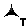
\includegraphics[height=2\baselineskip]{../images/cursorFloatOverTrack.png}\qquad
 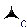
\includegraphics[height=2\baselineskip]{../images/cursorFloatOverClip.png}\qquad
 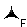
\includegraphics[height=2\baselineskip]{../images/cursorFloatOverFade.png}\qquad
 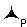
\includegraphics[height=2\baselineskip]{../images/cursorFloatOverPlugin.png}
 \caption{Der Mauszeiger ändert sich je nach Objekt, über welchem er sich befindet. Von links nach rechts: Spur (Track), Clip, Ein-, Ausblendebereich (Fade), Plugin.}
 \label{fig_cursor}
\end{figure}
